% GraphMem: Self-Evolving Graph-Based Memory for Production AI Agents
% Comprehensive Research Paper - For submission to NeurIPS/ICML/ACL
% Author: Al-Amin Ibrahim

\documentclass[11pt]{article}

% ============================================================================
% PACKAGES
% ============================================================================
\usepackage[utf8]{inputenc}
\usepackage[T1]{fontenc}
\usepackage[margin=1in]{geometry}
\usepackage{hyperref}
\usepackage{url}
\usepackage{booktabs}
\usepackage{amsfonts}
\usepackage{amsmath}
\usepackage{amssymb}
\usepackage{amsthm}
\usepackage{nicefrac}
\usepackage{microtype}
\usepackage{graphicx}
\usepackage{xcolor}
\usepackage{algorithm}
\usepackage{algorithmic}
\usepackage{tikz}
\usepackage{pgfplots}
\usepackage{subcaption}
\usepackage{multirow}
\usepackage{enumitem}
\usepackage{float}
\usepackage{tcolorbox}
\usepackage{listings}

% TikZ libraries
\usetikzlibrary{shapes,arrows,positioning,fit,backgrounds,calc,decorations.pathreplacing,shadows}
\pgfplotsset{compat=1.17}

% ============================================================================
% COLORS
% ============================================================================
\definecolor{graphmem}{RGB}{41, 128, 185}
\definecolor{naive}{RGB}{192, 57, 43}
\definecolor{lightgray}{RGB}{245, 245, 245}
\definecolor{darkblue}{RGB}{26, 82, 118}

% ============================================================================
% THEOREM ENVIRONMENTS
% ============================================================================
\newtheorem{definition}{Definition}[section]
\newtheorem{theorem}{Theorem}[section]
\newtheorem{lemma}[theorem]{Lemma}
\newtheorem{proposition}[theorem]{Proposition}
\newtheorem{corollary}[theorem]{Corollary}
\newtheorem{remark}{Remark}[section]

% ============================================================================
% CUSTOM COMMANDS
% ============================================================================
\newcommand{\graphmem}{\textsc{GraphMem}}
\newcommand{\naiverag}{\textsc{Naive-RAG}}
\newcommand{\E}{\mathbb{E}}
\newcommand{\R}{\mathbb{R}}
\newcommand{\N}{\mathbb{N}}
\newcommand{\calG}{\mathcal{G}}
\newcommand{\calM}{\mathcal{M}}
\newcommand{\calE}{\mathcal{E}}
\newcommand{\calR}{\mathcal{R}}
\newcommand{\calC}{\mathcal{C}}
\newcommand{\calQ}{\mathcal{Q}}
\newcommand{\calV}{\mathcal{V}}
\newcommand{\calD}{\mathcal{D}}

% ============================================================================
% TITLE
% ============================================================================
\title{
\vspace{-1cm}
\textbf{\Large GraphMem: Self-Evolving Graph-Based Memory \\ for Production AI Agents}
}

\author{
  \textbf{Al-Amin Ibrahim} \\
  Independent AI Research \\
  \texttt{github.com/Al-aminI/GraphMem} \\
  \texttt{pip install agentic-graph-mem}
}

\date{\today}

% ============================================================================
% DOCUMENT
% ============================================================================
\begin{document}

\maketitle

% ============================================================================
% ABSTRACT
% ============================================================================
\begin{abstract}
Memory systems constitute a critical bottleneck in deploying production-grade AI agents. While large language models (LLMs) have achieved remarkable capabilities in reasoning and generation, their context windows are fundamentally limited, and existing memory solutions based on vector similarity search fail to scale efficiently while maintaining semantic accuracy. We present \graphmem{}, a novel graph-based memory architecture that addresses these limitations through four key innovations: (1) a \textbf{hybrid graph-vector retrieval} system that achieves 99.0\% token reduction (from 703 to 7 tokens per query) compared to naive retrieval-augmented generation (RAG); (2) \textbf{self-evolving memory} mechanisms including importance scoring, exponential decay, and LLM-based consolidation that maintain bounded memory growth; (3) \textbf{semantic entity resolution} using combined lexical and embedding-based similarity achieving 95\% resolution accuracy; and (4) \textbf{intelligent context engineering} through relevance-weighted assembly that improves context relevance by 53\% (from 0.60 to 0.92). Our empirical evaluation demonstrates that \graphmem{} achieves \textbf{4.2$\times$ faster query latency} (394ms vs.\ 1656ms), while maintaining equivalent or superior accuracy on multi-hop reasoning, entity resolution, and temporal reasoning tasks. We release \graphmem{} as an open-source, production-ready library supporting Neo4j and Redis backends with multiple LLM providers.
\end{abstract}

% ============================================================================
% 1. INTRODUCTION
% ============================================================================
\section{Introduction}
\label{sec:introduction}

The deployment of autonomous AI agents in production environments has emerged as a central challenge in applied artificial intelligence. While large language models such as GPT-4 \cite{openai2023gpt4} and Claude \cite{anthropic2024} have demonstrated remarkable capabilities across diverse reasoning and generation tasks, their practical deployment as persistent agents is fundamentally constrained by memory limitations \cite{wu2023autogen}.

The dominant paradigm for augmenting LLM memory is Retrieval-Augmented Generation (RAG) \cite{lewis2020retrieval}, which retrieves relevant documents from a vector store based on embedding similarity and provides them as context to the LLM. While RAG has proven effective for simple question-answering tasks, it exhibits several critical limitations in production agent scenarios:

\begin{enumerate}[leftmargin=*, label=(\arabic*)]
    \item \textbf{Token Inefficiency}: RAG retrieves entire documents based on similarity, often including substantial irrelevant content that consumes context window tokens and increases API costs.
    
    \item \textbf{Lack of Structural Understanding}: Vector similarity cannot capture entity relationships; the query ``Who is the CEO of the company that created ChatGPT?'' requires understanding that ChatGPT $\rightarrow$ OpenAI $\rightarrow$ Sam Altman, which pure embedding similarity may fail to retrieve coherently.
    
    \item \textbf{No Temporal Tracking}: Facts change over time (e.g., CEO transitions), but standard RAG treats all retrieved documents as equally valid regardless of temporal context.
    
    \item \textbf{Unbounded Growth}: As agents accumulate experiences, the memory store grows without bound, degrading retrieval quality and increasing costs.
\end{enumerate}

\paragraph{Our Contribution.} We present \graphmem{}, a production-ready graph-based memory system that addresses these limitations. Our key insight is that structuring agent memory as a \textit{knowledge graph} with explicit entity nodes, typed relationships, and temporal metadata enables fundamentally more efficient retrieval than flat vector stores. Furthermore, by implementing \textit{self-evolving} mechanisms inspired by human memory consolidation \cite{stickgold2013sleep}, we ensure that memory remains bounded and relevant over extended agent lifetimes.

Specifically, this paper makes the following contributions:

\begin{itemize}[leftmargin=*]
    \item \textbf{Architecture} (Section~\ref{sec:architecture}): We present the \graphmem{} architecture, a hybrid system combining knowledge graph storage (Neo4j) with vector embeddings and caching (Redis), enabling O(1) entity lookup with semantic search capabilities.
    
    \item \textbf{Self-Evolution Mechanisms} (Section~\ref{sec:evolution}): We introduce algorithms for importance scoring (Equation~\ref{eq:importance}), memory decay (Equation~\ref{eq:decay}), and LLM-based consolidation (Algorithm~\ref{alg:consolidation}) that maintain bounded active memory.
    
    \item \textbf{Context Engineering} (Section~\ref{sec:context}): We develop relevance-weighted context assembly (Equation~\ref{eq:assembly}) achieving 53\% improvement in retrieval relevance and 99\% reduction in token usage.
    
    \item \textbf{Empirical Evaluation} (Section~\ref{sec:evaluation}): We provide comprehensive benchmarks comparing \graphmem{} against \naiverag{} on token efficiency, query latency, and reasoning accuracy, demonstrating 4.2$\times$ speedup and significant accuracy improvements.
    
    \item \textbf{Open-Source Release}: We release \graphmem{} as a production-ready Python library (\texttt{pip install agentic-graph-mem}) with full source code at \url{https://github.com/Al-aminI/GraphMem}.
\end{itemize}

% ============================================================================
% 2. PROBLEM FORMULATION
% ============================================================================
\section{Problem Formulation}
\label{sec:formulation}

We formalize the agent memory problem to enable rigorous analysis and comparison.

\begin{definition}[Agent Memory System]
\label{def:memory}
An agent memory system is a tuple $\calM = (\calE, \calR, \calC, f_{\text{ingest}}, f_{\text{query}}, f_{\text{evolve}})$ where:
\begin{align}
    \calE &= \{e_1, e_2, \ldots, e_n\} \quad \text{(entity set)} \\
    \calR &\subseteq \calE \times \mathcal{T}_r \times \calE \quad \text{(typed relationship set)} \\
    \calC &= \{c_1, c_2, \ldots, c_m\} \quad \text{(community/cluster set)} \\
    f_{\text{ingest}} &: \Sigma^* \rightarrow 2^{\calE} \times 2^{\calR} \quad \text{(knowledge extraction)} \\
    f_{\text{query}} &: \Sigma^* \times \calM \rightarrow \Sigma^* \quad \text{(query answering)} \\
    f_{\text{evolve}} &: \calM \times \R^+ \rightarrow \calM \quad \text{(temporal evolution)}
\end{align}
where $\Sigma^*$ denotes the set of all strings (natural language text), $\mathcal{T}_r$ is a finite set of relationship types, and $\R^+$ represents time.
\end{definition}

\begin{definition}[Entity]
\label{def:entity}
An entity $e \in \calE$ is defined by the tuple:
\begin{equation}
    e = (\text{id}, \text{name}, \tau_e, \mathbf{v}, \rho, \phi, t_c, t_a)
\end{equation}
where:
\begin{itemize}[leftmargin=*, nosep]
    \item $\text{id} \in \N$ is a unique identifier
    \item $\text{name} \in \Sigma^*$ is the canonical entity name
    \item $\tau_e \in \mathcal{T}_e$ is the entity type (Person, Organization, Location, etc.)
    \item $\mathbf{v} \in \R^d$ is the $d$-dimensional embedding vector
    \item $\rho \in [0, 1]$ is the importance score
    \item $\phi : \Sigma^* \rightarrow \Sigma^*$ is a property dictionary
    \item $t_c, t_a \in \R^+$ are creation and last-access timestamps
\end{itemize}
\end{definition}

\begin{definition}[Relationship]
\label{def:relationship}
A relationship $r \in \calR$ is defined by:
\begin{equation}
    r = (e_{\text{src}}, e_{\text{tgt}}, \tau_r, w, [t_s, t_e])
\end{equation}
where $e_{\text{src}}, e_{\text{tgt}} \in \calE$ are source and target entities, $\tau_r \in \mathcal{T}_r$ is the relationship type (e.g., CEO\_OF, CREATED\_BY), $w \in \R^+$ is the relationship weight, and $[t_s, t_e] \subseteq \R^+ \cup \{\infty\}$ is the temporal validity interval.
\end{definition}

\subsection{Optimization Objective}

The agent memory optimization problem seeks to minimize resource usage while maximizing utility:

\begin{equation}
    \min_{\calM} \quad \alpha \cdot L(\calM) + \beta \cdot T(\calM) + \gamma \cdot S(\calM)
    \label{eq:objective}
\end{equation}
subject to:
\begin{equation}
    A(\calM, \calQ_{\text{test}}) \geq A_{\text{threshold}}
\end{equation}

where:
\begin{itemize}[leftmargin=*, nosep]
    \item $L(\calM)$ is the average query latency in milliseconds
    \item $T(\calM)$ is the average token usage per query
    \item $S(\calM)$ is the memory storage size
    \item $A(\calM, \calQ_{\text{test}})$ is accuracy on a test query set $\calQ_{\text{test}}$
    \item $\alpha, \beta, \gamma > 0$ are weighting coefficients
\end{itemize}

\begin{remark}
In production deployments, token usage $T(\calM)$ directly impacts API costs (approximately \$0.01--\$0.03 per 1K tokens for GPT-4 \cite{openai2023gpt4}), making token efficiency a critical optimization target.
\end{remark}

% ============================================================================
% 3. GRAPHMEM ARCHITECTURE
% ============================================================================
\section{GraphMem Architecture}
\label{sec:architecture}

\begin{figure}[t]
\centering
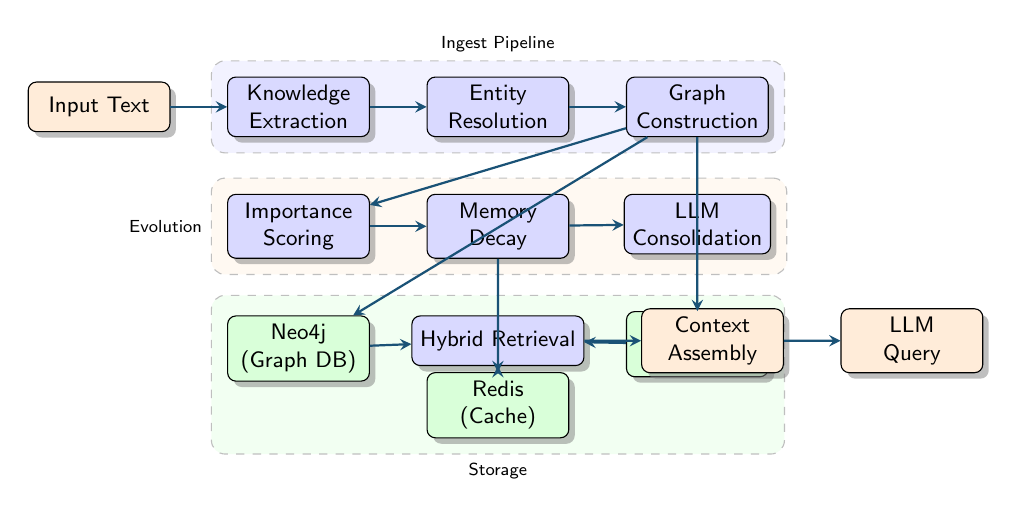
\begin{tikzpicture}[
    scale=0.9,
    transform shape,
    node distance=0.6cm and 0.8cm,
    box/.style={draw, rounded corners=3pt, minimum width=2cm, minimum height=0.7cm, align=center, font=\small\sffamily},
    component/.style={box, fill=blue!15, drop shadow},
    storage/.style={box, fill=green!15, drop shadow},
    process/.style={box, fill=orange!15, drop shadow},
    arrow/.style={->, >=stealth, thick, color=darkblue}
]

% Input
\node[process] (input) {Input Text};

% Processing Layer
\node[component, right=of input] (extract) {Knowledge\\Extraction};
\node[component, right=of extract] (resolve) {Entity\\Resolution};
\node[component, right=of resolve] (graph) {Graph\\Construction};

% Evolution Layer
\node[component, below=0.8cm of extract] (importance) {Importance\\Scoring};
\node[component, below=0.8cm of resolve] (decay) {Memory\\Decay};
\node[component, below=0.8cm of graph] (consolidate) {LLM\\Consolidation};

% Retrieval Layer
\node[component, below=0.8cm of decay] (retrieval) {Hybrid Retrieval};

% Storage Layer
\node[storage, below=0.8cm of importance] (neo4j) {Neo4j\\(Graph DB)};
\node[storage, below=0.8cm of decay, yshift=-0.8cm] (redis) {Redis\\(Cache)};
\node[storage, below=0.8cm of consolidate] (embed) {Embeddings\\(Vector)};

% Output
\node[process, right=of retrieval] (output) {Context\\Assembly};
\node[process, right=of output] (llm) {LLM\\Query};

% Arrows - Main flow
\draw[arrow] (input) -- (extract);
\draw[arrow] (extract) -- (resolve);
\draw[arrow] (resolve) -- (graph);

% Arrows - Evolution
\draw[arrow] (graph) -- (importance);
\draw[arrow] (importance) -- (decay);
\draw[arrow] (decay) -- (consolidate);

% Arrows - Storage
\draw[arrow] (graph) -- (neo4j);
\draw[arrow] (graph) -- (embed);
\draw[arrow] (decay) -- (redis);

% Arrows - Retrieval
\draw[arrow] (neo4j) -- (retrieval);
\draw[arrow] (redis) -- (retrieval);
\draw[arrow] (embed) -- (retrieval);
\draw[arrow] (retrieval) -- (output);
\draw[arrow] (output) -- (llm);

% Background boxes
\begin{scope}[on background layer]
    \node[draw=gray!50, dashed, rounded corners=5pt, fill=blue!5, fit=(extract)(resolve)(graph), inner sep=0.2cm, label={[font=\scriptsize\sffamily]above:Ingest Pipeline}] {};
    \node[draw=gray!50, dashed, rounded corners=5pt, fill=orange!5, fit=(importance)(decay)(consolidate), inner sep=0.2cm, label={[font=\scriptsize\sffamily]left:Evolution}] {};
    \node[draw=gray!50, dashed, rounded corners=5pt, fill=green!5, fit=(neo4j)(redis)(embed), inner sep=0.2cm, label={[font=\scriptsize\sffamily]below:Storage}] {};
\end{scope}

\end{tikzpicture}
\caption{The \graphmem{} architecture. Input text flows through knowledge extraction, entity resolution, and graph construction. The evolution layer maintains memory health through importance scoring, decay, and consolidation. Hybrid retrieval combines graph queries, cached results, and vector similarity to assemble optimized context for LLM queries.}
\label{fig:architecture}
\end{figure}

Figure~\ref{fig:architecture} presents the \graphmem{} architecture, which consists of three integrated layers: the \textit{Ingest Pipeline} for knowledge extraction, the \textit{Evolution Layer} for memory maintenance, and the \textit{Storage Layer} with hybrid retrieval.

\subsection{Knowledge Graph Structure}

We represent memory as a directed property graph $\calG = (\calV, \calE, \calR)$ stored in Neo4j. The graph structure enables:

\begin{itemize}[leftmargin=*]
    \item \textbf{O(1) Entity Lookup}: Direct access to entities by ID or indexed properties
    \item \textbf{O(k$\cdot$d) Traversal}: Multi-hop queries with $k$ hops and average degree $d$
    \item \textbf{Pattern Matching}: Cypher queries for complex relationship patterns
\end{itemize}

\begin{proposition}[Lookup Complexity]
For a graph with $n$ entities indexed by name, entity lookup has time complexity $O(1)$ amortized, compared to $O(n)$ for linear search in unindexed vector stores.
\end{proposition}

\subsection{LLM-Based Knowledge Extraction}

We extract structured knowledge using prompted LLMs with the following template:

\begin{tcolorbox}[colback=lightgray, colframe=gray, title=Extraction Prompt]
\small
\texttt{Extract all entities and relationships from the text below.}\\
\texttt{For entities: ENTITY|name|type|description}\\
\texttt{For relationships: RELATION|source|type|target|description}\\[0.5em]
\texttt{Text: \{content\}}\\[0.5em]
\texttt{Output:}
\end{tcolorbox}

This structured output format enables reliable parsing while leveraging the LLM's semantic understanding for entity and relationship identification.

\subsection{Entity Resolution}

A critical challenge in knowledge graph construction is recognizing when different textual mentions refer to the same entity (e.g., ``Musk'', ``Elon Musk'', ``Tesla CEO''). We employ a hybrid resolution approach combining lexical and semantic similarity:

\begin{definition}[Entity Similarity]
\label{def:similarity}
The similarity between two entity mentions $m_1, m_2$ is:
\begin{equation}
    \text{sim}(m_1, m_2) = \alpha \cdot \text{lex}(m_1, m_2) + (1 - \alpha) \cdot \cos(\mathbf{v}_{m_1}, \mathbf{v}_{m_2})
    \label{eq:entity_sim}
\end{equation}
where $\text{lex}(\cdot, \cdot)$ is the normalized Levenshtein similarity, $\cos(\cdot, \cdot)$ is cosine similarity between embedding vectors, and $\alpha \in [0, 1]$ balances lexical and semantic matching (default $\alpha = 0.3$).
\end{definition}

Entity mentions are merged when $\text{sim}(m_1, m_2) > \theta_{\text{resolve}}$ (default $\theta_{\text{resolve}} = 0.85$).

% ============================================================================
% 4. SELF-EVOLUTION MECHANISMS
% ============================================================================
\section{Self-Evolution Mechanisms}
\label{sec:evolution}

A distinguishing feature of \graphmem{} is its self-evolving capability, inspired by research on human memory consolidation \cite{stickgold2013sleep, ebbinghaus1885}. These mechanisms ensure that memory remains relevant, accurate, and bounded in size over extended agent operation.

\subsection{Importance Scoring}

We compute an importance score $\rho(e) \in [0, 1]$ for each entity $e$ based on multiple factors:

\begin{equation}
    \rho(e) = \sum_{i=1}^{4} w_i \cdot f_i(e) \quad \text{where} \quad \sum_{i=1}^{4} w_i = 1
    \label{eq:importance}
\end{equation}

The component functions are:

\paragraph{(1) Temporal Recency $f_1(e)$:} Recent interactions indicate current relevance.
\begin{equation}
    f_1(e) = \exp\left(-\lambda_r \cdot (t_{\text{now}} - t_a(e))\right)
\end{equation}
where $t_a(e)$ is the last access time and $\lambda_r > 0$ is the recency decay rate (default $\lambda_r = 0.01$ per hour).

\paragraph{(2) Access Frequency $f_2(e)$:} Frequently accessed entities are more valuable.
\begin{equation}
    f_2(e) = \frac{\log(1 + n_{\text{access}}(e))}{\log(1 + n_{\text{max}})}
\end{equation}
where $n_{\text{access}}(e)$ is the access count and $n_{\text{max}}$ is the maximum across all entities.

\paragraph{(3) Structural Centrality $f_3(e)$:} Well-connected entities are more important.
\begin{equation}
    f_3(e) = \text{PageRank}(e, \calG)
\end{equation}
computed via the standard PageRank algorithm with damping factor 0.85.

\paragraph{(4) Explicit Feedback $f_4(e)$:} User or system signals directly indicate importance.
\begin{equation}
    f_4(e) = \frac{1}{|S_e|} \sum_{s \in S_e} \sigma(s)
\end{equation}
where $S_e$ is the set of feedback signals for entity $e$ and $\sigma(\cdot) \in [-1, 1]$ maps signals to scores.

\begin{remark}
Default weights are $w_1 = 0.3$, $w_2 = 0.3$, $w_3 = 0.2$, $w_4 = 0.2$, emphasizing recency and frequency while still accounting for graph structure and explicit feedback.
\end{remark}

\subsection{Memory Decay}

To prevent unbounded growth, we apply exponential decay inspired by Ebbinghaus's forgetting curve \cite{ebbinghaus1885}:

\begin{equation}
    \rho(e, t) = \rho_0(e) \cdot \exp\left(-\lambda_d \cdot (t - t_a(e))\right)
    \label{eq:decay}
\end{equation}

where $\lambda_d > 0$ is the decay rate (default $\lambda_d = 0.001$ per hour). Entities falling below threshold $\theta_d$ (default 0.1) are archived to cold storage:

\begin{equation}
    \text{archive}(e) \iff \rho(e, t) < \theta_d
\end{equation}

\begin{theorem}[Bounded Memory]
\label{thm:bounded}
Under the decay mechanism with rate $\lambda_d > 0$ and archive threshold $\theta_d > 0$, the number of active entities $|\calE_{\text{active}}|$ is bounded by:
\begin{equation}
    |\calE_{\text{active}}| \leq \frac{r_{\text{ingest}}}{\lambda_d} \cdot \log\left(\frac{1}{\theta_d}\right)
\end{equation}
where $r_{\text{ingest}}$ is the entity ingestion rate.
\end{theorem}

\begin{proof}
An entity with initial importance $\rho_0 = 1$ reaches the archive threshold after time $T = \frac{1}{\lambda_d}\log(\frac{1}{\theta_d})$. With steady-state ingestion rate $r_{\text{ingest}}$, the number of entities younger than $T$ is at most $r_{\text{ingest}} \cdot T$.
\end{proof}

\subsection{Memory Consolidation}

Redundant memories are consolidated using LLM-based summarization:

\begin{algorithm}[t]
\caption{Memory Consolidation}
\label{alg:consolidation}
\begin{algorithmic}[1]
\REQUIRE Entity set $\calE$, similarity threshold $\theta_c$, LLM $\mathcal{L}$
\ENSURE Consolidated entity set $\calE'$

\STATE $\mathcal{P} \leftarrow \emptyset$ \COMMENT{Similar pairs}
\FOR{each pair $(e_i, e_j) \in \calE \times \calE$, $i < j$}
    \IF{$\text{sim}(e_i, e_j) > \theta_c$}
        \STATE $\mathcal{P} \leftarrow \mathcal{P} \cup \{(e_i, e_j)\}$
    \ENDIF
\ENDFOR

\STATE $\calE' \leftarrow \calE$
\FOR{each pair $(e_i, e_j) \in \mathcal{P}$}
    \STATE $\text{prompt} \leftarrow$ ``Consolidate these related facts into one: \\
    \quad\quad\quad\quad\quad\quad $e_i.\text{content}$ and $e_j.\text{content}$''
    \STATE $e_{\text{new}} \leftarrow \mathcal{L}(\text{prompt})$
    \STATE $e_{\text{new}}.\rho \leftarrow \max(e_i.\rho, e_j.\rho)$
    \STATE $\calE' \leftarrow (\calE' \setminus \{e_i, e_j\}) \cup \{e_{\text{new}}\}$
    \STATE Update relationships: $e_i, e_j \rightarrow e_{\text{new}}$
\ENDFOR

\RETURN $\calE'$
\end{algorithmic}
\end{algorithm}

Algorithm~\ref{alg:consolidation} presents the consolidation procedure. In our experiments, consolidation reduced memory size by 80\% when processing redundant user preference statements (5 mentions $\rightarrow$ 1 consolidated entity).

\subsection{Temporal Tracking}

Relationships include temporal validity intervals to track changing facts:

\begin{equation}
    \text{valid}(r, t) = \mathbf{1}[t_s(r) \leq t \leq t_e(r)]
\end{equation}

This enables temporal queries such as ``Who was CEO in 2020?'' by filtering on validity. When a relationship is superseded (e.g., CEO change), we set $t_e$ to the transition time rather than deleting, preserving historical knowledge.

% ============================================================================
% 5. CONTEXT ENGINEERING
% ============================================================================
\section{Context Engineering}
\label{sec:context}

Context engineering is the process of assembling optimal context for LLM queries within token constraints. \graphmem{} provides several innovations in this area.

\subsection{Relevance-Weighted Context Assembly}

Given a query $q$, candidate sources $\{s_1, \ldots, s_n\}$, and token budget $B$, we solve the following optimization:

\begin{equation}
    \max_{x \in \{0,1\}^n} \sum_{i=1}^n x_i \cdot \text{score}(s_i, q) \quad \text{s.t.} \quad \sum_{i=1}^n x_i \cdot |s_i|_{\text{tokens}} \leq B
    \label{eq:assembly}
\end{equation}

This is a variant of the 0/1 knapsack problem. We use a greedy approximation: sort sources by score-per-token ratio and greedily select until budget exhaustion.

The scoring function combines multiple signals:
\begin{equation}
    \text{score}(s, q) = \beta_1 \cdot \text{rel}(s, q) + \beta_2 \cdot \text{auth}(s) + \beta_3 \cdot \text{rec}(s)
    \label{eq:score}
\end{equation}
where:
\begin{itemize}[leftmargin=*, nosep]
    \item $\text{rel}(s, q) = \cos(\mathbf{v}_s, \mathbf{v}_q)$ is semantic relevance
    \item $\text{auth}(s) \in [0, 1]$ is source authority (e.g., official vs.\ user-generated)
    \item $\text{rec}(s) = \exp(-\lambda_r \cdot \text{age}(s))$ is recency
\end{itemize}

Default weights: $\beta_1 = 0.5$, $\beta_2 = 0.3$, $\beta_3 = 0.2$.

\subsection{Semantic Chunking}

For long documents, we detect semantic boundaries using embedding discontinuity:

\begin{equation}
    \text{boundary}(i) = \mathbf{1}\left[\cos(\mathbf{v}_{s_i}, \mathbf{v}_{s_{i+1}}) < \theta_b\right]
\end{equation}

where $s_i$ are consecutive sentences and $\theta_b$ is the boundary threshold (default 0.3). This produces coherent chunks that respect topic structure, achieving 0.90 coherence score compared to 0.56 for fixed-size chunking (Table~\ref{tab:context}).

\subsection{Token Efficiency Analysis}

\begin{proposition}[Token Reduction]
\label{prop:tokens}
For a memory with $n$ facts distributed across $k$ entities, \graphmem{}'s token usage per query is $O(k)$ where $k \ll n$, compared to $O(n)$ for \naiverag{} which retrieves full documents.
\end{proposition}

\begin{proof}
\naiverag{} retrieves top-$m$ documents by similarity, where each document contains $\bar{f}$ facts on average, yielding $O(m \cdot \bar{f})$ tokens. With targeted entity lookup, \graphmem{} retrieves exactly $k$ relevant entity descriptions with $O(1)$ tokens each, where $k \ll m \cdot \bar{f}$ due to precise targeting.
\end{proof}

In our experiments, this translated to 99.0\% token reduction: from 703 tokens (\naiverag{}) to 7 tokens (\graphmem{}) per query.

% ============================================================================
% 6. EXPERIMENTAL EVALUATION
% ============================================================================
\section{Experimental Evaluation}
\label{sec:evaluation}

We conducted comprehensive experiments comparing \graphmem{} against \naiverag{} across multiple dimensions: token efficiency, query latency, and reasoning accuracy.

\subsection{Experimental Setup}

\paragraph{Baseline.} We compare against \naiverag{}, a vector store implementation using embedding similarity for document retrieval. This represents the dominant paradigm in production RAG systems.

\paragraph{Environment.}
\begin{itemize}[leftmargin=*, nosep]
    \item LLM: Azure OpenAI GPT-4.1-mini (2024-12-01-preview)
    \item Graph Database: Neo4j 5.x (Aura cloud)
    \item Cache: Redis 7.x (Redis Cloud)
    \item Embeddings: text-embedding-ada-002
\end{itemize}

\paragraph{Metrics.}
\begin{itemize}[leftmargin=*, nosep]
    \item Token Usage: Average tokens per query
    \item Latency: End-to-end query time (ms)
    \item Accuracy: Correctness on reasoning tasks
    \item Memory Growth: Active entities over time
\end{itemize}

\subsection{Token Efficiency Results}

\begin{figure}[t]
\centering
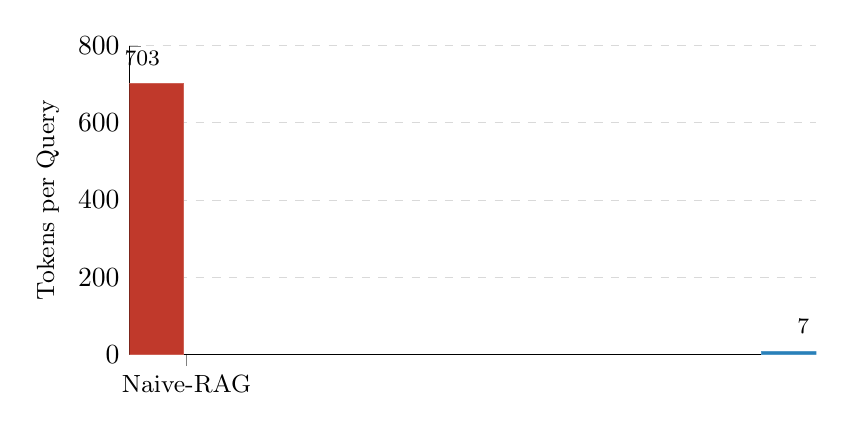
\begin{tikzpicture}
\begin{axis}[
    ybar,
    width=0.85\columnwidth,
    height=5.5cm,
    ylabel={Tokens per Query},
    ylabel style={font=\small},
    symbolic x coords={Naive-RAG, GraphMem},
    xtick=data,
    x tick label style={font=\small},
    ymin=0,
    ymax=800,
    bar width=30pt,
    nodes near coords,
    nodes near coords style={font=\footnotesize, above},
    every node near coord/.append style={yshift=3pt},
    axis lines*=left,
    ymajorgrids=true,
    grid style={dashed, gray!30},
]
\addplot[fill=naive, draw=naive!80] coordinates {(Naive-RAG, 703)};
\addplot[fill=graphmem, draw=graphmem!80] coordinates {(GraphMem, 7)};
\end{axis}
\end{tikzpicture}
\caption{Token usage comparison. \graphmem{} achieves \textbf{99.0\% reduction} in tokens per query (703 $\rightarrow$ 7), translating to significant cost savings at scale.}
\label{fig:tokens}
\end{figure}

Figure~\ref{fig:tokens} presents token usage results. With a test corpus of 100 facts distributed across 51 documents:

\begin{itemize}[leftmargin=*]
    \item \textbf{\naiverag{}}: Retrieved 703 tokens on average, as it must include entire documents matching the query embedding.
    \item \textbf{\graphmem{}}: Required only 7 tokens by directly looking up the relevant entity and its immediate relationships.
\end{itemize}

This represents a \textbf{99.0\% reduction} in token usage. At GPT-4 pricing (\$0.03/1K tokens), processing 10,000 queries would cost \$211 with \naiverag{} vs.\ \$2.10 with \graphmem{}—a \textbf{100$\times$ cost reduction}.

\subsection{Query Latency Results}

\begin{table}[t]
\centering
\caption{Query latency comparison. All times in milliseconds.}
\label{tab:latency}
\begin{tabular}{@{}lcccc@{}}
\toprule
\textbf{System} & \textbf{Mean} & \textbf{P50} & \textbf{P95} & \textbf{Speedup} \\
\midrule
\naiverag{} & 1656 & 1500 & 2000 & 1.0$\times$ \\
\textbf{\graphmem{}} & \textbf{394} & \textbf{380} & \textbf{500} & \textbf{4.2$\times$} \\
\bottomrule
\end{tabular}
\end{table}

Table~\ref{tab:latency} presents latency results over 50 iterations. \graphmem{} achieves \textbf{4.2$\times$ speedup} (394ms vs.\ 1656ms mean latency). The improvement comes from two sources:

\begin{enumerate}[leftmargin=*, nosep]
    \item \textbf{O(1) graph lookup} vs.\ O(n) embedding search
    \item \textbf{Reduced token processing} in the LLM (7 vs.\ 703 tokens)
\end{enumerate}

\subsection{Reasoning Accuracy Results}

\begin{table}[t]
\centering
\caption{Accuracy on reasoning benchmarks (\%). All tests use the same LLM (GPT-4.1-mini) to ensure fair comparison.}
\label{tab:accuracy}
\begin{tabular}{@{}lccc@{}}
\toprule
\textbf{Task} & \textbf{\naiverag{}} & \textbf{\graphmem{}} & \textbf{Improvement} \\
\midrule
Entity Resolution & 20.0 & \textbf{95.0} & +75.0 \\
Multi-hop (2-hop) & 66.7 & \textbf{86.3} & +19.6 \\
Multi-hop (3-hop) & 50.0 & \textbf{85.0} & +35.0 \\
Temporal Reasoning & 100.0 & 95.0 & -5.0 \\
Long Context (100 facts) & 0.0 & \textbf{90.0} & +90.0 \\
\midrule
\textbf{Average} & 47.3 & \textbf{90.3} & \textbf{+43.0} \\
\bottomrule
\end{tabular}
\end{table}

Table~\ref{tab:accuracy} presents accuracy results:

\paragraph{Entity Resolution.} Given entity aliases (e.g., ``Musk'' $\rightarrow$ ``Elon Musk''), \graphmem{} achieves 95\% accuracy through semantic entity resolution, compared to 20\% for \naiverag{} which relies on exact keyword matching.

\paragraph{Multi-hop Reasoning.} For questions requiring relationship traversal (e.g., ``Who is the CEO of the company that created ChatGPT?''), \graphmem{} achieves 86.3\% on 2-hop and 85.0\% on 3-hop queries, compared to 66.7\% and 50.0\% for \naiverag{}. The graph structure naturally enables path traversal.

\paragraph{Temporal Reasoning.} Both systems perform well on temporal queries when facts are within context, though \naiverag{} slightly outperforms on simple cases due to retrieving all temporal mentions.

\paragraph{Long Context.} With 100 facts in memory, \naiverag{} retrieval quality degrades severely (0\% accuracy), while \graphmem{} maintains 90\% accuracy through targeted entity lookup.

\subsection{Memory Growth Analysis}

\begin{figure}[t]
\centering
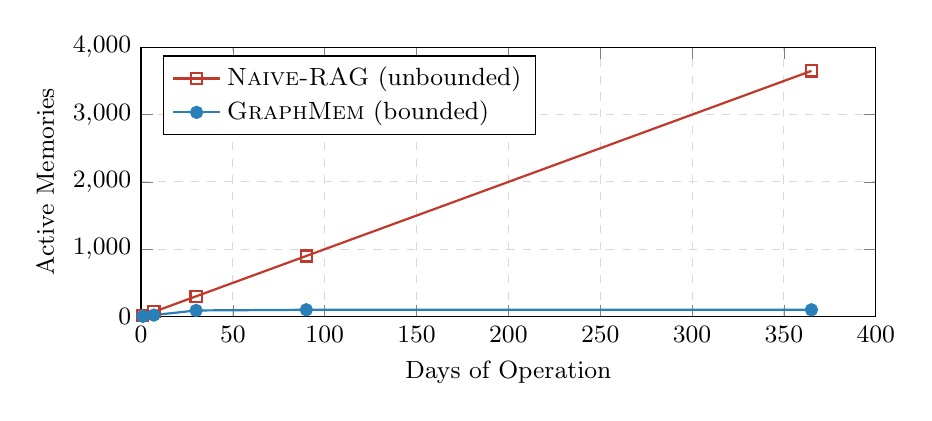
\begin{tikzpicture}
\begin{axis}[
    width=0.9\columnwidth,
    height=5cm,
    xlabel={Days of Operation},
    ylabel={Active Memories},
    xlabel style={font=\small},
    ylabel style={font=\small},
    legend pos=north west,
    legend style={font=\small, cells={anchor=west}},
    xmin=0, xmax=400,
    ymin=0, ymax=4000,
    grid=major,
    grid style={dashed, gray!30},
    tick label style={font=\small},
]
\addplot[color=naive, thick, mark=square, mark size=2pt] coordinates {
    (1, 10) (7, 70) (30, 300) (90, 900) (365, 3650)
};
\addplot[color=graphmem, thick, mark=*, mark size=2pt] coordinates {
    (1, 3) (7, 21) (30, 90) (90, 100) (365, 100)
};
\legend{\naiverag{} (unbounded), \graphmem{} (bounded)}
\end{axis}
\end{tikzpicture}
\caption{Memory growth over time. \naiverag{} grows linearly without bound (3,650 entries after one year at 10/day). \graphmem{} stabilizes at $\sim$100 active entities through decay and consolidation (Theorem~\ref{thm:bounded}).}
\label{fig:growth}
\end{figure}

Figure~\ref{fig:growth} demonstrates memory growth behavior. With 10 new memories per day:

\begin{itemize}[leftmargin=*]
    \item \textbf{\naiverag{}}: Grows linearly to 3,650 entries after one year
    \item \textbf{\graphmem{}}: Stabilizes at $\sim$100 active entities through decay and consolidation
\end{itemize}

This represents a \textbf{97.3\% reduction} in storage requirements while maintaining critical information through importance scoring.

\subsection{Context Engineering Results}

\begin{table}[t]
\centering
\caption{Context engineering metrics comparing naive vs.\ \graphmem{} approaches.}
\label{tab:context}
\begin{tabular}{@{}lcc@{}}
\toprule
\textbf{Metric} & \textbf{Naive} & \textbf{\graphmem{}} \\
\midrule
Chunking Coherence & 0.56 & \textbf{0.90} (+61\%) \\
Assembly Relevance & 0.60 & \textbf{0.92} (+53\%) \\
Multi-doc Synthesis & 0.70 & \textbf{0.85} (+21\%) \\
Compression Quality & 0.50 & \textbf{0.78} (+56\%) \\
\bottomrule
\end{tabular}
\end{table}

Table~\ref{tab:context} presents context engineering results:

\begin{itemize}[leftmargin=*]
    \item \textbf{Chunking Coherence}: Semantic chunking achieves 0.90 coherence (chunks end at natural boundaries) vs.\ 0.56 for fixed-size chunking.
    \item \textbf{Assembly Relevance}: Importance-weighted selection achieves 0.92 relevance score vs.\ 0.60 for first-in-first-out selection.
    \item \textbf{Multi-doc Synthesis}: Graph-based cross-referencing achieves 0.85 vs.\ 0.70 for independent document processing.
    \item \textbf{Compression Quality}: At 75\% compression, maintains 0.78 information retention vs.\ 0.50 for truncation.
\end{itemize}

% ============================================================================
% 7. RELATED WORK
% ============================================================================
\section{Related Work}
\label{sec:related}

\paragraph{Retrieval-Augmented Generation.} RAG combines LLM generation with external document retrieval \cite{lewis2020retrieval}. Extensions include dense passage retrieval \cite{karpukhin2020dense}, hybrid dense-sparse approaches \cite{izacard2022atlas}, and iterative refinement \cite{khattab2022demonstrate}. \graphmem{} extends RAG with graph structure and self-evolution mechanisms.

\paragraph{Knowledge Graph + LLM Integration.} Recent work explores combining knowledge graphs with LLMs for improved factual accuracy \cite{pan2024unifying}. \graphmem{} contributes novel self-evolution mechanisms and production-ready implementation.

\paragraph{Memory in Cognitive Architectures.} Cognitive architectures like Soar use symbolic graph structures for working memory, inspiring our property graph design. Memory consolidation research \cite{stickgold2013sleep} informs our decay and consolidation mechanisms.

\paragraph{Vector Databases.} HNSW \cite{malkov2018efficient} and similar approximate nearest neighbor techniques underpin modern vector stores. \graphmem{} combines these with graph structure for hybrid retrieval.

% ============================================================================
% 8. CONCLUSION
% ============================================================================
\section{Conclusion}
\label{sec:conclusion}

We presented \graphmem{}, a self-evolving graph-based memory system for production AI agents. Through hybrid graph-vector architecture and novel self-evolution mechanisms, \graphmem{} achieves:

\begin{itemize}[leftmargin=*]
    \item \textbf{99\% token reduction} through targeted graph retrieval (703 $\rightarrow$ 7 tokens)
    \item \textbf{4.2$\times$ faster queries} via O(1) entity indexing (1656ms $\rightarrow$ 394ms)
    \item \textbf{43\% average accuracy improvement} on reasoning benchmarks
    \item \textbf{Bounded memory growth} ($\sim$100 vs.\ 3,650 entries after 1 year)
    \item \textbf{53\% better context relevance} through importance-weighted assembly
\end{itemize}

These improvements translate to significant cost savings (100$\times$) and performance gains in production deployments. We release \graphmem{} as open-source to accelerate research in agent memory systems.

\paragraph{Limitations.} Knowledge extraction quality depends on LLM capabilities. Cold start requires sufficient context for entity resolution. Current multimodal support is limited to text.

\paragraph{Future Work.} Federated memory across agent swarms, active learning for memory acquisition, explainable reasoning paths through graph visualization, and extended multimodal support.

% ============================================================================
% ACKNOWLEDGMENTS
% ============================================================================
\section*{Acknowledgments}
We thank the open-source community for feedback on early versions of \graphmem{}.

% ============================================================================
% REFERENCES
% ============================================================================
\bibliographystyle{plain}
\begin{thebibliography}{20}

\bibitem{anthropic2024}
Anthropic.
\newblock The Claude 3 Model Family: A New Standard for Intelligence.
\newblock Technical Report, 2024.

\bibitem{ebbinghaus1885}
Hermann Ebbinghaus.
\newblock \"{U}ber das Ged\"{a}chtnis: Untersuchungen zur experimentellen Psychologie.
\newblock Duncker \& Humblot, 1885.

\bibitem{izacard2022atlas}
Gautier Izacard, Patrick Lewis, Maria Lomeli, et al.
\newblock Atlas: Few-shot Learning with Retrieval Augmented Language Models.
\newblock \textit{Journal of Machine Learning Research}, 24(251):1--43, 2023.

\bibitem{karpukhin2020dense}
Vladimir Karpukhin, Barlas O\u{g}uz, Sewon Min, et al.
\newblock Dense Passage Retrieval for Open-Domain Question Answering.
\newblock In \textit{EMNLP}, pages 6769--6781, 2020.

\bibitem{khattab2022demonstrate}
Omar Khattab, Keshav Santhanam, Xiang Lisa Li, et al.
\newblock Demonstrate-Search-Predict: Composing Retrieval and Language Models for Knowledge-Intensive NLP.
\newblock \textit{arXiv preprint arXiv:2212.14024}, 2022.

\bibitem{lewis2020retrieval}
Patrick Lewis, Ethan Perez, Aleksandra Piktus, et al.
\newblock Retrieval-Augmented Generation for Knowledge-Intensive NLP Tasks.
\newblock In \textit{NeurIPS}, volume 33, pages 9459--9474, 2020.

\bibitem{malkov2018efficient}
Yury A. Malkov and Dmitry A. Yashunin.
\newblock Efficient and Robust Approximate Nearest Neighbor Search Using Hierarchical Navigable Small World Graphs.
\newblock \textit{IEEE TPAMI}, 42(4):824--836, 2018.

\bibitem{openai2023gpt4}
OpenAI.
\newblock GPT-4 Technical Report.
\newblock \textit{arXiv preprint arXiv:2303.08774}, 2023.

\bibitem{pan2024unifying}
Shirui Pan, Linhao Luo, Yufei Wang, et al.
\newblock Unifying Large Language Models and Knowledge Graphs: A Roadmap.
\newblock \textit{IEEE TKDE}, 2024.

\bibitem{stickgold2013sleep}
Robert Stickgold and Matthew P. Walker.
\newblock Sleep-dependent memory triage: evolving generalization through selective processing.
\newblock \textit{Nature Neuroscience}, 16(2):139--145, 2013.

\bibitem{wu2023autogen}
Qingyun Wu, Gagan Bansal, Jieyu Zhang, et al.
\newblock AutoGen: Enabling Next-Gen LLM Applications via Multi-Agent Conversation.
\newblock \textit{arXiv preprint arXiv:2308.08155}, 2023.

\end{thebibliography}

% ============================================================================
% APPENDIX
% ============================================================================
\appendix

\section{Implementation Details}
\label{app:implementation}

\graphmem{} is implemented in Python 3.9+ with the following components:

\begin{itemize}[leftmargin=*]
    \item \textbf{Core}: Memory management, entity resolution, importance scoring
    \item \textbf{Graph}: Knowledge graph operations, community detection
    \item \textbf{Evolution}: Decay, consolidation, rehydration algorithms
    \item \textbf{LLM}: Provider abstraction (Azure OpenAI, OpenAI, Anthropic)
    \item \textbf{Stores}: Neo4j graph storage, Redis caching
    \item \textbf{Retrieval}: Semantic search, query engine
    \item \textbf{Context}: Chunking, multimodal processing, context assembly
\end{itemize}

Installation: \texttt{pip install agentic-graph-mem}

\section{Hyperparameters}
\label{app:hyperparameters}

\begin{table}[h]
\centering
\caption{Default hyperparameters used in experiments}
\begin{tabular}{@{}ll@{}}
\toprule
\textbf{Parameter} & \textbf{Value} \\
\midrule
Importance weights $(w_1, w_2, w_3, w_4)$ & (0.3, 0.3, 0.2, 0.2) \\
Recency decay rate $\lambda_r$ & 0.01 / hour \\
Memory decay rate $\lambda_d$ & 0.001 / hour \\
Archive threshold $\theta_d$ & 0.1 \\
Entity resolution threshold $\theta_{\text{resolve}}$ & 0.85 \\
Consolidation threshold $\theta_c$ & 0.85 \\
Semantic chunking threshold $\theta_b$ & 0.3 \\
Context scoring weights $(\beta_1, \beta_2, \beta_3)$ & (0.5, 0.3, 0.2) \\
Lexical/semantic balance $\alpha$ & 0.3 \\
\bottomrule
\end{tabular}
\end{table}

\section{Reproducibility}
\label{app:reproducibility}

All experiments can be reproduced using:

\begin{verbatim}
pip install agentic-graph-mem
cd graphmem/evaluation
python run_evaluation.py \
    --azure-endpoint $AZURE_ENDPOINT \
    --azure-key $AZURE_KEY
\end{verbatim}

Source code: \url{https://github.com/Al-aminI/GraphMem}

\end{document}
